% arara: pdflatex: { synctex: yes }
% arara: makeindex: { style: ctuthesis }
%% arara: bibtex

%\listfiles


%\PassOptionsToPackage{cp1250}{inputenc}

% The class takes all the key=value arguments that \ctusetup does,
% and couple more: draft and oneside
\documentclass[twoside]{ctuthesis}

\usepackage{natbib}

\makeatletter
\edef\mytoday{\expandafter\@gobbletwo\the\year\ifnum\month<10 0\fi\the\month\ifnum\day<10 0\fi\the\day}
\makeatother

% LaTeX logo with better kerning in sf bf font
\makeatletter
\newcommand\LaTeX@lmss@bx{L\kern-.33em{\sbox\z@ T\vboxto\ht\z@{\hbox{\check@mathfonts\fontsize\sf@size\z@\math@fontsfalse\selectfont A}\vss}}\kern-.15em\TeX}
\DeclareRobustCommand\myLaTeX{%
	\ifcsname LaTeX@\f@family @\f@series\endcsname
		\csname LaTeX@\f@family @\f@series\endcsname
	\else
		\LaTeX
	\fi
}

\ctusetup{
%	preprint = {\ctuverlog \\ ctuman \mytoday},
	mainlanguage = english,
%	titlelanguage = english,
%	otherlanguages = {czech},
	% title-czech = {Manuál ke třídě ctuthesis pro {\myLaTeX}},
	title-english = {NLP Trolls},
	doctype-english = {Bachelor thesis},
%	xfaculty = F4,
%	department-czech = {Katedra matematiky},
%	department-english = {Department of Mathematics},
	author = {Luka Peraica },
	supervisor = {Ing. Radek Mařík, CSc.},
%	supervisor-address = {Ústav X, \\ Uliční 5, \\ Praha 99},
	keywords-czech = {manuál, závěrečnná práce, \LaTeX},
	keywords-english = {manual, degree project, \LaTeX},
	day = 16,
	month = 4,
	year = 2024,
%	list-of-figures = false,
%	list-of-tables = false,
%	monochrome = true,
%	savetoner = true,
	pkg-listings = true,
	ctulstbg = none,
%	layout-short = true,
%	pkg-hyperref = false,
}

\ctuprocess

% Theorem declarations, this is the reasonable default, anybody can do what they wish.
% If you prefer theorems in italics rather than slanted, use \theoremstyle{plainit}
\theoremstyle{plain}
\newtheorem{theorem}{Theorem}[chapter]
\newtheorem{corollary}[theorem]{Corollary}
\newtheorem{lemma}[theorem]{Lemma}
\newtheorem{proposition}[theorem]{Proposition}

\theoremstyle{definition}
\newtheorem{definition}[theorem]{Definition}
\newtheorem{example}[theorem]{Example}
\newtheorem{conjecture}[theorem]{Conjecture}

\theoremstyle{note}
\newtheorem*{remark*}{Remark}
\newtheorem{remark}[theorem]{Remark}

% Marginpars used as navigation aids.
\usepackage{mparhack} 

\newcommand\indexmp[1]{{\sffamily\bfseries#1}}

\ExplSyntaxOn
\cs_new:Nn \ctuman_domarginpar:n {
	\marginpar
	[ \raggedleft \footnotesize \sffamily #1 ]
	{ \raggedright \footnotesize \sffamily #1 }
}
\cs_generate_variant:Nn \ctuman_domarginpar:n { x }
\DeclareDocumentCommand\ctump{m}{
	\clist_set:Nn \ctuman_temp_clist { #1 }
	\ctuman_domarginpar:x { \clist_use:Nnnn \ctuman_temp_clist { \\ } { \\ } { \\ } }
	\clist_map_inline:Nn \ctuman_temp_clist { \index{##1|indexmp} }
	\ignorespaces
}
\ExplSyntaxOff

\usepackage{graphicx}

% Abstract in Czech
\begin{abstract-czech}
V záplavě mnoha zdrojů a množství mediálních zpráv není jednoduché se zorientovat i pro profesionální mediální analytiky. 
Výrazem demokracie je i možnost se ke zprávám vyjadřovat a tříbit si názory v diskusních příspěvcích dílčích zpráv. 
Diskuse však vytváří prostor i pro osoby, jejichž cílem je z rozmanitých důvodu diskuse narušovat a překrucovat. 
Cílem práce je vytvořit komponenty systému, který umožní sledovat linie vývoje tématu a identifikovat příspěvky narušitelů, 
tzv. trollů.\end{abstract-czech}

% Abstract in English
\begin{abstract-english}
	
\end{abstract-english}

% Acknowledgements / Podekovani
\begin{thanks}
	We thank the CTU in Prague for being a~very good \emph{alma mater}.
\end{thanks}

% Declaration / Prohlaseni
\begin{declaration}
	I declare that this work is all my own work and I have cited all sources I have
	used in the bibliography.

\medskip

	Prague, \monthinlanguage{title} \ctufield{day}, \ctufield{year}

\vspace*{2cm}

	Prohlašuji, že jsem předloženou práci vypracoval samostatně, a že jsem uvedl veškerou použitou literaturu.

\medskip

	V Praze, \ctufield{day}.~\monthinlanguage{second}~\ctufield{year}
\end{declaration}

\usepackage{url}

\usepackage{tabularx,array}
\usepackage{multirow} % Required for \multirow command
\usepackage{booktabs}  

\usepackage{mathtools,amssymb}

% A savebox for typesetting listings in the titles
\newsavebox{\myboxa}

%\newcommand*\symbO{$\color{red}\bowtie$}
\newcommand*\symbO{\raisebox{0.5\height}{\scalebox{0.7}{\color{red}${\vartriangleright}\mkern-6mu{\vartriangleleft}$}}}
\newcommand*\symbM{\raisebox{0.5\height}{\scalebox{0.7}{\color{red}${\blacktriangleright}\mkern-6mu{\blacktriangleleft}$}}}
\newcommand*\itemO{\item\leavevmode\kern-0.33em\symbO}
\newcommand*\itemM{\item\leavevmode\kern-0.33em\symbM}



\begin{document}

% We actually don't want inline listings to have a background color
\renewcommand \ctulstsep{0pt}

% \ctuclsname for typesetting the class' name
\newcommand\ctuclsname{\leavevmode\unhcopy\ctuclsnamebox}
\newsavebox\ctuclsnamebox
\begin{lrbox}{\ctuclsnamebox}
\ctulst!ctuthesis!
\end{lrbox}

\maketitle

% ========================================== CHAPTER 1 INTRODUCTION ==============================
\chapter{Introduction}

\section{Problem Statement}
\par
The way humans communicate and interact has changed dramatically in the age of the internet. Social media sites, forums and comment sections have become primary spaces for people to share ideas, debate issues and engage in public discourse. These online discussion platforms allow individual from different backgrounds to express their opinions and be part of conversations easily than ever before. However, while online discussions create opportunities for connecting people and sharing information, they also come with major challenges like the spread of misinformation, the polarization of society and the spread of large scale disruptive behavior.\par

Understanding how these platforms shape opinion is essential in the modern day. As in today's flood of diverse media sources and information, even professional media analysts find it challenging to navigate and filter reliable information. A key aspect of democracy is the ability to express opinions and refine perspectives through discussions. Today most of such discussion happens online on social media platforms like Twitter, Facebook and Reddit which have gained a powerful influence on public opinion the shaping political outcomes~\cite{Bennett2012DigitalMedia}. This importance and ubiquity of online discussions can also make them targets for individuals whose goal is to disrupt and manipulate conversations for various reasons.\par

\section{Defining Online Trolling}
To address the negative consequences of disruptive online behavior, it is important to define one its most prevalent forms: online trolling. Online trolling is a deliberate act intended to provoke, deceive, or disrupt online conversations. According to Coles and West~\cite{Coles2016}, trolling involves actions meant to annoy, frustrate, or engage others in pointless disputes. Similarly, Golf-Papez and Veer~\cite{GolfPapez2017DontFeedTheTroll} define trolling as ''deliberate, deceptive, and mischievous attempts to provoke reactions from other users''.\par

The term ''trolling'' itself was originally borrowed from fishing slang, where it referred to dragging a baited line through the water to catch fish. In the online context, the term seems to have first been used  in the 1990s on the USET discussion system where some users would deliberately create posts designed to trigger angry corrections from newbie users who weren't aware of such pracitces.\par

Then there is a second definition for the word ''troll'', which is also quite relevant to the perception of online trolls and perhaps for most people the first connotation that comes to mind. This definition refers to a troll as a large, ugly creature from folklore, often depicted brutish ogre. The word ''troll'' is derived from the Old Norse word ''troll'', which means ''giant'' or ''ogre''. In this context, the term evokes an image of a monstrous being that lurks in the shadows, waiting to pounce on unsuspecting victims. And while the term trolling originated from the early bait posts, related to the fishing term, over time the the character and label of the ''troll'' developed, which is more closely related to the folklore definition. This shift in meaning reflects the evolution of online trolling from more light-hearted baiting and joking to a label for a malicious character lurking on the internet.\cite{Demsar2021}\par

While some forms of trolling may seem harmless or playful, others can escalate into targeted harassment, misinformation campaigns, and efforts to manipulate public opinion.\par
People engage in trolling for various reasons, from simply seeking amusement from the activity to pushing political or ideological agendas. Studies indicate that personality traits like psychopathy, narcissism, and Machiavellianism are often linked to trolling behavior~\cite{Buckels2014TrollsWantToHaveFun}. Additionally research has shown that certain psychological factors also contribute to the online trolling phenomena, such as the ''online disinhibition effect''. This theory suggests that people act more aggressively online because they feel anonymous and free from real-world consequences~\cite{Suler2004}. The combination of these factors makes online discussions particularly fertile ground for antisocial behavior. \par

Beyond individual psychology trolls also exploit the techonological factor of the discussions, particularly social media algorithms that focus on engagement above all else. Effectively playing into the algorithm allows them to more easily and effectively spread divisive content and manipulate conversations~\cite{GolfPapez2017DontFeedTheTroll}.\par

\section{Impacts of Trolling}
Trolling negatively affects both honest users and the discussion as a whole. Those targeted by trolls often experience stress, anxiety, and frustration, which can discourage them from engaging in future conversations. Trolling not only harms individual well-being but also degrades the quality of discussions. As user trust is eroded and people become more skeptical of digital interactions a toxic environment is created where constructive engagement becomes difficult~\cite{GolfPapez2017DontFeedTheTroll}.\par

On a larger scale trolling can have significant consequences, particularly when it is used as a toll for political manipulation. State-sponsored troll campaigns have been used to spread propaganda, influence elections, and undermine public trust in media~\cite{Bradshaw2017TroopsTrolls}. One of the most well-known exaples is the Russian \textit{Internet Research Agency} (IRA), which ran large-scale trolling operations during the 2016 U.S. presidential election between Hillary Clinton and Donald Trump. These trolls used fake accounts to post divisive content and manipulate public discourse~\cite{Linvill2020IRATrolls}. Similar use of trolling in political campaigns and foreign influence operations has been documented across the world, demonstrating the severity and importance of addressing the issue.\par

This thesis aims to identify and analyze behavior of trolls in online discussions. Specifically, it will explore different NLP techniques for troll detection, including stylometry, topic modeling, deep learning, and transformer models. The goal is to identify harmful contributions and contributors to online discussions and to explore possibilites for further research in this area.\par

% ========================================== CHAPTER 2 NLP =====================
\chapter{Natural Language Processing}
Given the impact of disruptive trolls on online discourse and society at large, research efforts have focused on developing techniques to better understand, detect and mitigate their activity. This chapter explores the methods used to analyze and identify trolling behavior particularly through Natural Language Processing (NLP). It covers key approaches such as stylometry, sentiment analysis, and topic modelling.\par

\section{Stylometry}

Stylometry is the discipline of analyzing writing style to uncover patterns, identify authors, and extract meaningful details from texts~\cite{Mosteller1964Federalist}~\cite{Pascucci2020Misogyny}. The term was introduced in 1890 by the Polish philosopher Wincenty Lutosławski, who applied it to analyze Plato's works~\cite{Lutoslawski1898}. In the context of this thesis,  stylometry involves the use of automated techniques to analyze linguistic traits that distinguish authors based on their unique writing patterns.\par
The underlying assumption in stylometry is that an author's choices are influenced by sociological factors, such as age, gender, and education level, as well as psychological factors, like personality and native language proficiency~\cite{Daelemans2013Explanation}. This assumption can be extended to groups of authors, especially those who may share common objectives or adhere to specific guidelines, such as state-sponsored trolls, or display similar behavioral patterns as seen among ordinary trolls. These individual or collective choices can manifest as identifiable stylistic features within texts, which computational models can analyze to detect trolling behavior.
Stylometric analyses typically examine lexical choices like vocabulary richness, syntactic elements including sentence structure and grammatical complexity~\cite{Sari2018Features}, and semantic dimensions, such as sentiment and thematic consistency~\cite{PerezRosas2018Stylometry}. Extracting and evaluating these features allows machine learning classifiers to differentiate between regular users and trolls based on their distinctive linguistic signatures.\par

\subsection{Stylometry in Literature}

An example of stylometry applied to troll detection is presented in the work of Machová \textit{et al.}~\cite{Machova2021Algorithms}. The paper examines troll detection in Slovak Facebook discussions on COVID-19 by combining shallow stylometric cues with engagement and affective information.  From roughly 2,500 manually labelled comments they extract length-based metrics (character and word counts, average word length), orthographic signals (capital-letter and digit frequency), and eight sentiment/provocativeness categories, and enrich these with interaction metadata such as the number of “likes.”  Classical classifiers-including SVM, Multinomial Naïve Bayes (MNB) and logistic regression-are trained on bag-of-words and TF-IDF representations.  The MNB model that integrates stylometric, affective and metadata features achieves the best balance, reaching 0.92 recall for the troll class, while an SVM attains perfect precision (1.00) at the cost of markedly lower recall.  Their results confirm that stylistic signals are informative but deliver the highest performance when fused with complementary sentiment and platform-level features, rather than being relied upon in isolation.

In another paper an example of stylometry applied to fake news detection is presented in the work of Pérez-Rosas et al.~\cite{PerezRosas2018Stylometry}. They used a variety of stylometric features, including n-grams, punctuation frequency, readability metrics and syntactic features. They also incorporated psycholingustic features extracted from the LIWC lexicon which categorize words into various psychological categories. LIWC features capture psychological aspets of a text such as emotional tone or cognitive processes, potentially revealing underlying psychological differences between fake and legitimate news writers. A linear SVM classifier was trained on these features to differentiate between fake and legitimate news articles. Their results showed that stylometric features can be effective for the task, achieving accuracies of up to 76\% which outperformed two human annotators. The analysis uncovered distinct linguistic patterns in fake news, such as increased use of social and positive words, a focus on present and future actions, and a higher prevalence of adverbs, verbs, and punctuation marks. 

% In another paper, Kandasamy et at.~\cite{Kandasamy2021COVID} proposed a deep learning framework for sentiment analysis of COVID-19-related tweets. Their approach used an N-gram stacked autoencoder to capture text features. These features were then processed by a set of classifiers-decision trees, support vector machines, random forests, and k-nearest neighbors. The highest accuracy was achieved using an ensemble model that combined all of these classifiers, this method achieved an accuracy of 87.75\%. The study demonstrated that using n-grams greatly improved the classification of negative sentiment, an emotion that was prevalent during the pandemic.\par

Though stylometry has proven useful for text classification, recent advancements in large language models and their potential for misuse might pose a substantial challenge to its efficacy. As demonstrated by Schuster et al.~\cite{Schuster2020}, stylmoetry may struggle to differentiate between human-written and machine-generated text. In their study they find that while a state-of-the-art stylometry-based classifier could effectively detect the presence of machine-generated text within human-written content, it struggled to discern the truthfulness of the generated text.  For instance, even a single auto-generated sentence within a longer human-written text was easily detectable, but the veracity of that sentence remained largely undecidable.  Additionally, even a relatively weak LM could produce statement inversions that evaded detection by the stylometry-based model.\par

These findings collectively highlight stylometry's potential for detecting hidden manipulation in online text, although recent advancements in language generation models present new challenges. It is also imporatnt to note that to achieve good results stylometric features weren't used on their own but along with others like meta data (like counts, followers) or sentiemnt analysis. \par

\section{Sentiment Analysis}
Sentiment analysis is a method of determining the emotional tone of text, which can be achieved using lexicon-based methods, machine learning, or deep learning approaches. It identifies positive, negative, neutral, or ambivalent tones in text.\par

\subsection{Sentiment Analysis in Troll Detection}
The use of sentiment analysis has been explored as one of the methods used of troll detection. Jiang et al.~\cite{Jiang2021Sentiment} for example explored the use of sentiment analysis for troll detection on the Chinese social media platform Weibo.  They employed a Word2Vec model trained on a dataset of Weibo comments to generate word embeddings. These embeddings were then used to calculate sentiment scores, incorporating features such as happiness, anger, disgust, and fear. The sentiment was used along with meta features such as the location of a comment in a thread or its like count to train XGBoost and SVM models for the troll detection task. The approach proved effective with the XGBoost model achieving an accuracy of up to 89\% and SVM up to 87\%.\par
In a related study, Machová et al.~\cite{Machova2022Comparison} investigated the detection of suspicious reviewers in online discussions, focusing on trolls. . Their lexicon-based approach analyzed the polarity of comments to identify trolls. It was based on the tendency of trolls to express extreme opinions that oppose the general sentiment of the discussion. They compared this approach with a Convolutional Neural Network (CNN) model, finding that both performed similarly on text data, achieving accuracies of 0.95 and 0.959, respectively.  The study also employed machine learning methods, such as Support Vector Machines (SVM), using non-textual features like comment karma, likes, and dislikes. With the SVM model they achieved an accuracy of 0.986.

\section{Topic Detection}
Topic detection is another essential NLP technique used to analyze and interpret corpora of text. It identifies main topics in large amounts of text and groups conversations based on these topics. This can help us understand conversation patterns and recognize signs of disruptive behavior. Trolls often move discussions off-topic, introduce controversial subjects, or focus repeatedly on divisive issues. We can analyze the kinds of topics a user engages with and how they behave within those topics to find clues about their intentions and their role in discussions.\par

\section{Transformer Models}
%TODO: Vysvletit vice do hlobky? -attention, encoder-decoder, pre-training etc., matika?
In recent years, Transformer models have emerged as the state-of-the-art approach for a wide range of NLP tasks. Introduced by First introduced by Vaswani et al. in 2017~\cite{Vaswani2017}, Transformers offer a new way for machines to understand and generate language. Unlike earlier methods, they are designed to efficiently capture relationships and patterns within text, even over long passages. Their ability to handle large amounts of data and to adapt to complex language structures has made them a key tool in modern NLP applications. In this section, we will introduce the basic ideas behind Transformer models.\par

The key innovation of Transformer models is the use of self-attention mechanisms. Instead of processing text word by word like earlier models, Transformers can consider all words in a sentence at once, deciding how much attention each word should pay to others. This allows the model to capture complex patterns and dependencies across long texts, making it very powerful for understanding the both the context and meaning of language.\par

An important reason for the success of Transformer models is that they are typically very large models pre-trained on massive datasets. Many of these datasets are multilingual, meaning that the models learn from several languages at once. As a result, we can often use the same embedding space for different languages, and the knowledge gained in one language can transfer to some extent to others. This makes pre-trained Transformers especially valuable when dealing with multilingual or cross-lingual data.\par

One of the most influential Transformer-based models for natural language understanding is BERT (Bidirectional Encoder Representations from Transformers). Introduced by Devlin et al. in 2018~\cite{Devlin2018}, BERT builds on the Transformer encoder architecture and is pre-trained on large text corpora using masked language modeling and next sentence prediction tasks. Unlike traditional language models that read text from left to right, BERT is deeply bidirectional, meaning it learns information from both the left and right context at the same time. This bidirectional training allows BERT to capture richer information about language, making it highly effective for downstream tasks like text classification, question answering, and sentiment analysis.

\subsection{Transformer Models in Troll Detection}
The paper MetaTroll proposed MetaTroll, a few-shot troll detection framework designed to adapt quickly to new state-sponsored influence campaigns using minimal labeled data. Their approach is based on a meta-learning framework and incorporates campaign-specific transformer adapters to tackle catastrophic forgetting, a common problem where models lose the ability to detect trolls from older campaigns after continual updates. MetaTroll outperformed traditional n-gram SVM baselines, achieving a 92.3\% F1-score in 5-shot scenarios and demonstrating strong cross-lingual capabilities.\cite{Tian2023}
Embeddings generated by transformer models have been shown to outperform static methods due to their ability to capture the contextual meanings of words. BERT based word embeddings outperformed static GloVe vectors are reached AUC scores of 0.924. The authors of the paper \cite{yilmaz2023} highlight how transformers can better cepture contextual nuances in language, which can be important for the task of troll classification, where language can be manipulative and deliberately deceptive.

In this thesis, we will attempt to leverage pre-trained Transformer such models as BERT and try to fine tune them for the troll detection task. The reasons for the choice of using Transformers will be outlined in the next chapter.\par

% ========================================== CHAPTER 4 PROPOSED METHOD ======================
\chapter{Dataset}

Before outlining the proposed method, I will first describe the dataset that forms the basis of our work. The properties of the dataset are important as it directly shape the choice of methods and defines the limitiations and the goals of the work. \par

\section{Main Dataset}
The dataset used in this thesis consists of user-generated comments collected from the discussion sections under news articles published on Novinky.cz, one of the largest Czech news portals. Each article on Novinky.cz includes a public comment section where users participate in discussions about the content presented. These discussions are often extensive, with some articles attracting hundreds of user comments.\par

In the Czech online media environment, it is generally recognized that the comment sections on major news sites, particularly on Novinky.cz for example, frequently serve as hotbeds for controversy and emotionally charged discourse. They are often perceived by the public as spaces where individuals express grievances, frustrations, and polarizing viewpoints, sometimes in ways that border on or cross into what could be described as abusive, manipulative or troll like behavior. This cultural context makes Novinky.cz a relevant and interesting setting for exploring how online discussions develop, especially where conversations become heated or emotionally charged.\par

For the purposes of this thesis, a large-scale dataset comprising approximately 350,000 comments posted by around 48,000 users was provided by Newton Media, a prominent media intelligence organization.\par 
% TODO: add time frame of collected data

Each data entry includes the following attributes:
\begin{itemize}
    \item \textbf{Comment content} - the full textual body of the comment.
    
    \item \textbf{Article metadata} - including the title and link to the article under which the comment was posted
    
    \item \textbf{Timestamp} - the date and time when the comment was published.
    
    \item \textbf{Author name} - full author name as collected from the discussion.
    
    \item \textbf{Sentiment label} - a sentiment category assigned by Newton Media, labeled as one of the following: \textit{Neutral}, \textit{Positive}, \textit{Negative}, or \textit{Ambivalent}.
\end{itemize}

A consideration for the work with this dataset is the nature of the comments. The comments in general seem to be mostly negative in tone and often emotionally charged, as can be seen by the distribution of setiment.

\begin{figure}[htbp]          
	\centering                 
	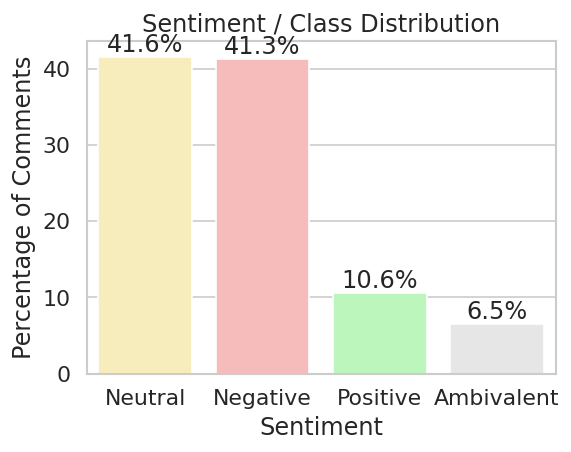
\includegraphics[scale=0.7]{figures/sentiment.png}
	\caption{Sentiment distribution of collected novinky.cz comments}    
	\label{fig:myplot}          
\end{figure}

A key challenge posed by this dataset is the absence of explicit troll/non-troll labels. Since there is no ground-truth annotation for trolling behavior, we cannot directly apply supervised classification methods. Because of this, we have to rely on unsupervised or semi-supervised techniques, such as clustering, topic modeling, or anomaly detection, to try to find patterns that may point to trolling based on how the comments are written and their sentiment. The lack of labeled data also makes it difficult to verify the accuracy or effectiveness of any classifications or patterns identified during experimentation. Without labeled data, we cannot easily measure how accurate our models are, and have to instead rely on manual checks and interpretation of the results.\par

\section{Additionall Datasets}

In addition to the primary dataset collected from Novinky.cz, several publicly available labeled datasets were also used in this thesis. They were collected from different platforms such as Twitter or Reddit and the majority are in English, although some include other languages as well. While they differ in context and language, they offer labeled examples that usd for pre-training of models for the later analysis of Czech online discussions.\par

\subsection{IRA Troll Tweets}
One of the external datasets used in this thesis is a collection of tweets linked to the Russian \textit{Internet Research Agency} (IRA), which was menitioned in the introductory chapter of the thesis. The dataset was published by FiveThirtyEight in connection with their article \textit{Why We're Sharing 3 Million Russian Troll Tweets}, and was originally collected by researchers from Clemson University. It contains nearly 3 million tweets posted between February 2012 and May 2018 by accounts identified by Twitter as being linked to the IRA, which were provided to the US Congress for investigation into 2016 presidential election interference. In total, the dataset includes 2,973,371 tweets from 2,848 Twitter handles. Most of the tweets are in English, but some are in other languages, including Russian or German. The dataset is publicly available and can be accessed through the FiveThirtyEight GitHub repository.\footnote{\url{https://github.com/fivethirtyeight/russian-troll-tweets/}}

\subsection{Information Operations Dataset}
Another external resource used in this thesis is a collection of labeled datasets for research on information operations (IOs), introduced by Seckin et al.~\cite{Seckin2024}. The full collection contains over 13 million posts from approximately 303,000 accounts. The dataset includes both verified IO posts and control data from legitimate accounts, covering 26 distinct manipulation campaigns originating from different countries. The data is organized first by one of 16 identified state actors, such as Russia, China, or even Catalonia, and then further subdivided into distinct operations. The IO posts were identified and released by major social media platforms including Twitter, Facebook, and Reddit, while the control data captures organic user discussions on similar topics within the same time frames.

\subsection{Non-troll Datasets}
In addition to the troll datasets several non-troll datasets were also collected to ensure availability of apolitical and organic user discussion.\par
The first non-troll dataset is the Civil Comments dataset, obtained from Hugging Face. It consists of public comments posted between 2015 and 2017 on approximately 50 English-language news sites. Each comment is labeled with values for toxicity, obscenity, and other attributes. For the purposes of this thesis, only comments labeled as non-toxic (toxicity score between 0 and 0.1) were used, which represent the majority of the dataset.\footnote{\url{https://huggingface.co/datasets/google/civil_comments}}\par

Additionally, a small dataset of celebrity tweets was obtained from Kaggle. This dataset consists of posts by well-known public figures providing examples of casual and generally non-political online communication.\footnote{\url{https://www.kaggle.com/datasets/abaghyangor/celebrity-tweets}}.\par

Finally, a custom dataset was manually created by scraping tweets from Czech public figures and politicians. A selected list of Twitter accounts was compiled, and 20 tweets were collected from each account. \par

% ========================================== CHAPTER 4 PROPOSED METHOD =====================
\chapter{Proposed Method}
In this chapter I will outline the proposed method for detecting troll-like behavior in online discussions. The core idea behind the method is the use of transformer-based models, specifically multilingual BERT based models, in a regression task designed to quantify the a users troll-like behavior. Instead of a binary classification task, the approach is to assign a user with a continous ''trolliness'' score, measured from 0 to 1.\par

\section{Motivation}
As the backbone of the method, I decided to use multilingual BERT based models, as they are trained across dozens of languages at once, which makes them a natural choice when trying to transfer knowledge from English or Russian troll datasets to Czech. Beyond their multilingual capabilities, BERT models are also able to capture and represent both syntactic and semantic relationships and dependencies within a text sequence. Instead of manually designing and extracting individual features like syntax counts, stylometric traits, sentiment scores, in theory BERT should be able to learn and encode much of this information into its embeddings and attention mechanism.\cite{Rogers2020}\par
A classical machine learning approach using stylometric and other features is not suitable for this task, due to the limitations of the datasets we are working with, which were mentioned above. However BERT should be able to capture similar semantic and syntactic knowledge while also being able to be used in our specific task with limited labeled data and multilingual datasets.\par
The motivation to use a regression task instead of a binary classification task is twofold. First, the main dataset of Czech comments lacks troll/non-troll labels, so standart supervised classification methods cannot be applied. Second, troll behavior isn't a straight forward binary state, but rather a spectrum of behavior, with users displaying varying degrees and different types of distruptive behavior.\par

\section{Data Collection and Preprocessing}
The first step of the method is the collection and preprocessing of the data. The raw text data is cleaned and preprocessed using basic text preprocessing techniques to normalize it to a certain extend across the different data sources. Each comment is then grouped according to its author, creating sets of comments for each user.\par
A key design decision in this work was to rate the trolliness at the user level, rather than at an individual comment level. This decision was based on the analysis and observations from the labeled troll datasets. A reccuring pattern was that many troll accounts did not only engage in disruptive and manipulative behavior all the time. Instead, in many cases trolls posted mostly ''normal'' content, perhaps to blend in with regular users, pushing their agenda more subdly in some posts and then only occasionally posting more overtly troll-like comments.\par
For this thesis we will exclude all users with fewer than 5 comments, as our aim is to try to find broader patterns of troll-like behavior not only one-off examples of offensive or provocative comments. We do this both for the initial training as well as when working with the target Czech dataset. While this discards about half of the users in the dataset, it is only a small fraction of the comments, about ten precent.\par
\begin{figure}[htbp]
	\centering
	% left image
	\begin{minipage}[b]{0.48\linewidth}
	  \centering
	  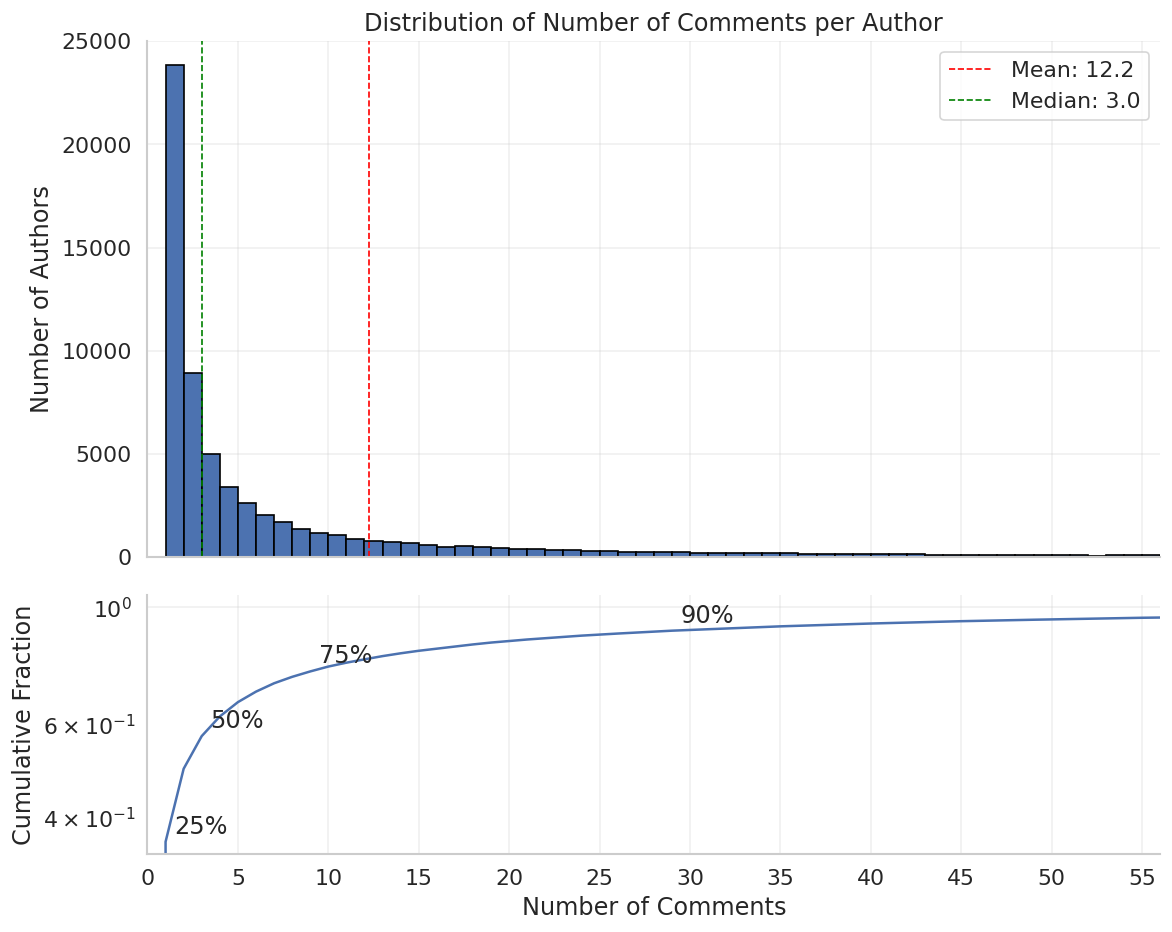
\includegraphics[width=\linewidth]{figures/comments_per_author.png}
	  \caption{First image}
	  \label{fig:left}
	\end{minipage}
	\hfill                  
	% right image
	\begin{minipage}[b]{0.48\linewidth}
	  \centering
	  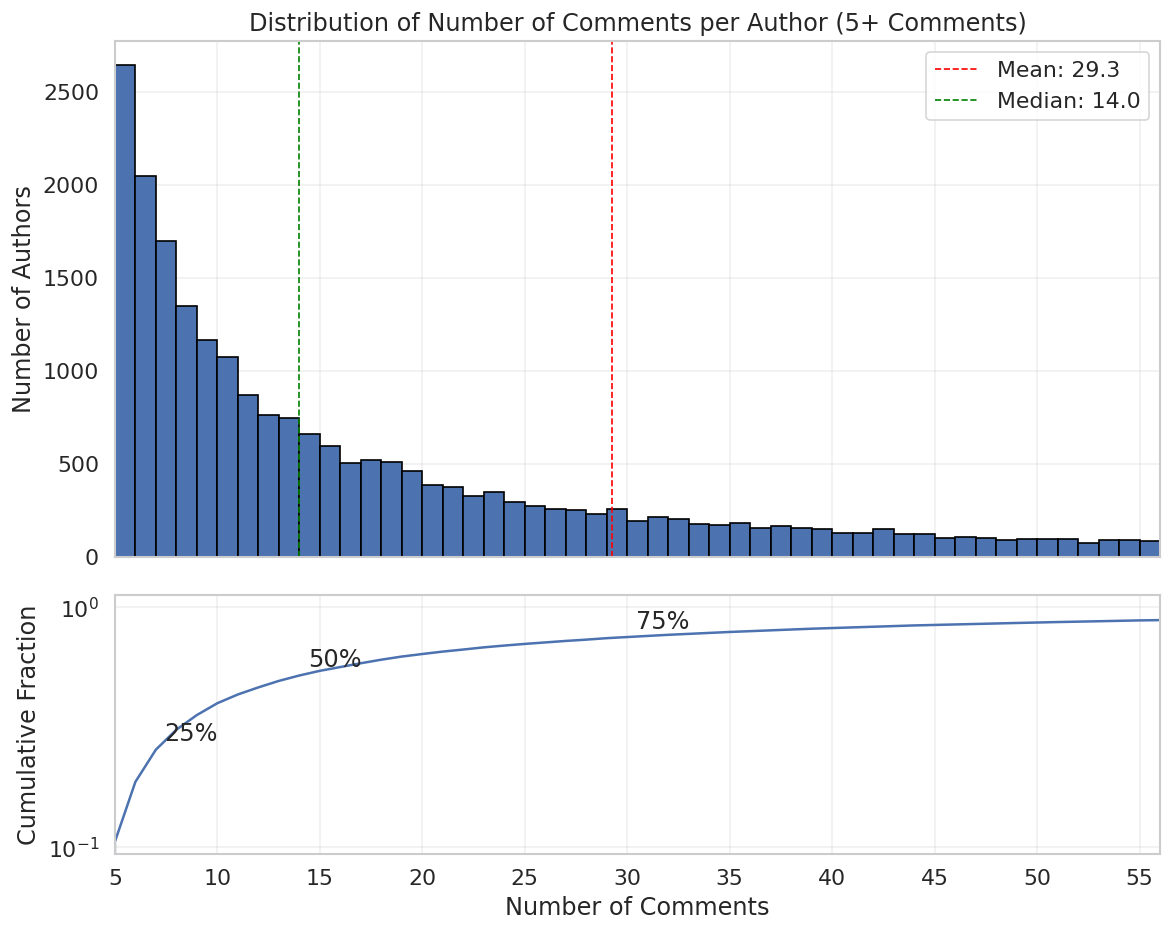
\includegraphics[width=\linewidth]{figures/comments_5_plus.png}
	  \caption{Second image}
	  \label{fig:right}
	\end{minipage}
	\caption{Distribution of comments per autor before and after filtering for 5+ comments}
	\label{fig:pair}
  \end{figure}

\section{Model Architecture}
The model architecture is designed in two levels: the comment level and the user level. At the comment level, each individual comment is first encoded using a pretrained multilingual BERT model. BERT processes the comments and produces fixed-length embeddings which capture both syntactic and semantic information.\par
At the user level, the embeddings of all the comments from a single user are aggregated. To combine all the comments into a single user-level vector, an attention mechanism is used. The attention mechanism allows the model to assign different importance to different comments, depending on how strongly they contribute to the the users trolliness. This allows the model to give greater influence to models which are more disruptive or otherwise suspicious when creating the final user representation.\par
Finally, a regression head is applied on top of the aggregated user-level embedding vector. The regression head consists of a feed-forward neural network, which outputs a the final coutninous trolliness score between 0 and 1. This score should reflect how similar a users behavior is to that of known trolls, rather than to give a hard classification.\par

\section{Training}
The training of the model is done in two steps. Larger training on the large labeled troll datasets from foreign domains, and a smaller fine-tune on manually annotated Czech comments from the target dataset.\par
The first training step includes the Russian IRA troll tweets, information operations datasets, and the non-troll datasets like Civil Comments. The training is done using a regression objective, where the model is trained to predict the trolliness of the users instead of their binary class.\par
Since the labeled training data comes from different domains and languages than our target Czech dataset, a second small fine-tuning step is performed. But first before starting this step, a lightweight adapter module was trained on the Czech comment corpus using a Masked Language Modeling (MLM) objective. This should help the model adapt for the Czech language domain better, but allows for the learned knowledge from the large foreign troll datasets to be kept.\par
After the initial training, the model is fine-tuned on a small set of manually annoated Czech user comments from our target dataset. This data was created by me, by exploring the users in the who were classified with high or low trolliness scores and high confidence during preliminary runs. This few-shot tuning step helps the model better adapt to our specific domain.\par


\section{Scoring}
Once the model is trained, it can be used to score the trolliness of users in the target dataset. For each user, all available comments are collected and grouped into batches of a fixed size. If a user has fewer comments than needed to fill a batch the comments are padded with empty comments. Each batch of comments is then passed through the model to generate a score. When a user has multple batches, the final trolliness score is calculated as the average over all batches.\par
The output of the model is then a continous trolliness score between 0 and 1. A binary predition can be obtained by applying a threshold. Additionally the model provides attention weights for individual comments, which how much each comment contributed to the final score and can be used for analysis and interpretation.\par


% ========================================== CHAPTER X  =====================
\chapter{Experiments}

\section{Baseline Comparison}
To evaluate the reasonability of the proposed method and how much a transfoer model really adds, we first reproduced a stylomtery-only baseline with the same trial/test/validation data splits used with the BERT model.
We used 5 stylometric features named in \cite{Machova2021Algorithms} - character count, word count, average word length, capital-letter ratio and digit ratio. We then trained two regressors on them a linar support-vector regressor (SVR) and a gradient-boosint regressor (GBR). We also added a stronger Term Frequency - Inverse Document Frequency (TF-IDF) based baseline with a representation of comments through 50000 unigrams and bigrams and fitting on a ridge regressor.\par

We will compare the training results of the models through their mean square error (MSE) and the coefficient of determination (the $R^2$ score). The mean square error (MSE) is a measure of the average squared difference between the predicted and actual values. A lower MSE indicates a better fit of the model to the data. 
% Mean-Squared Error
\[
\mathrm{MSE} = \frac{1}{n}\sum_{i=1}^{n}\bigl(y_i - \hat{y}_i\bigr)^2
\]
The $R^2$ score is a statistical measure of what share of the original variance of the data the model explains. To explain how it works let's first define the equations. First we define two sums of squares:\par
% --- Total Sum of Squares (TSS)
\[
\mathrm{TSS} \;=\; \sum_{i=1}^{n} \bigl(y_i - \bar{y}\bigr)^2,
\qquad
\bar{y} \;=\; \frac{1}{n}\sum_{i=1}^{n} y_i
\]

% --- Residual Sum of Squares (RSS)
\[
\mathrm{RSS} \;=\; \sum_{i=1}^{n} \bigl(y_i - \hat{y}_i\bigr)^2
\]

The $R^2$ score is then:
% R^2
% --- Coefficient of Determination (R^2)
\[
R^{2} \;=\; 1 \;-\; \frac{\mathrm{RSS}}{\mathrm{TSS}}
\]
\par

The $R^2$ score quantifes the proportion of total variance (TSS) that is left unexplained by the model's residuals (RSS).  A value of 1 indicates a perfect fit and 0 indicates that the model does not explain any of the variance in the data. A negative $R^2$ score indicates that the model performs worse than simply guessing the mean of the target variable.\par

\subsection{Evaluation of the Baseline}
With coarse stylometric features the SVR and GB regressors did not beat guessing the mean with a negative $R^2$ score and a MSE of about 0.26. This result is not too surprising as 5 features is much for the regression models to work with, but it shows notheless that few handpicked stylometric features are not enough. Extending to 50000 features (uni- and bi-gram counts) through TF-IDF improves $R^2$ score a lot, to 0.57 and has a mean square error of 0.09 but it still gets outperformed by the BERT model with a regression head which achieved a $R^2$ score of 0.65 and a MSE of 0.07. The results of the two best models TF-IDF and BERT are similiar, but the trained TF-IDF model cannot be used on other other language domains, whie the BERT model should be able to carry over some of its learned knowledge. The results of the model training and evaluation are shown in the table below.\par

\begin{table}[ht]
	\centering
	\caption{Author-level results on English train/test/val data.}
	\label{tab:en_author_results}
	\begin{tabular}{lccccc}
	  \hline
	  \textbf{Model} & \textbf{Features} &
	  \textbf{Val MSE} & \textbf{Val $R^{2}$} &
	  \textbf{Test MSE} & \textbf{Test $R^{2}$} \\
	  \hline
	  Linear SVR & 5 stylometric          & 0.260 & $-0.211$ & 0.260 & $-0.211$ \\
	  Ridge TF--IDF & 50\,000 1-2-grams   & 0.090 & 0.579   & 0.097 & 0.547    \\
	  DistilBERT & contextual   & \textbf{0.087} & \textbf{0.592} &
										   \textbf{0.082} & \textbf{0.618} \\
	  \hline
	\end{tabular}
\end{table}

We thus show that BERT achieves similar or better results than a stylometric model and we validate why we chose to use it.

\section{Further Experiments with BERT Model}

After preparing the dataset and implementing the proposed model, the next step is to evaluate and explore the models behavior. The goal of the experiemnts is to compare different training strategies and see how they do with trolliness scoring of the Czech dataset.\par
I compare three different versions of the model. 
\begin{itemize} 
	\item \textbf{Base model} - trained only on the foregin labeled troll datasets without any additional fine-tuning on Czech data. 
	\item \textbf{Base + Few-shot} - the base model further fine-tuned on a small manually annotated set of Czech users. 
	\item \textbf{Base + Adapter + Few-shot} - the base model with a Czech domain adapter trained first, followed by fine-tuning on the manually annotated Czech users. 
\end{itemize}
Each model is evaluated based on the distribution of predicted trolliness scores across users, manual review of selected user cases and performace on a small hand annotated test set.

\section{Adapter Training}
TODO vyhodnoceni treninku adapteru

\section{}
TODO ukazka vysledku a provnani modelu

\section{}
TODO, s regresnim trolliness score jako zakladem zkusit hledat korelace napriklad v clusterech topicu?. Pri prvni analyze jsem ale nenasel korelaci mezi trolovosit a napriklad poctem ruznych topicu do kterych uzivatel prispiva. 

\chapter{Annotation and Evaluation}

To help me work with the model and dataset, I created a simple annotation application. The main goal of the tool is to allows labeling of users from the Czech dataset and search for their comments. The app also shows the model's predicted trolliness scores and attention weights. The annotations can then be used both for few-shot fine-tuning and for manual exploration of the model's predictions.\par


\chapter{Conclusion}

\appendix

\printindex

\bibliographystyle{alpha} 
\bibliography{../sources/library.bib}

\end{document}